\documentclass[]{article}
%\setlength{\headheight}{13.59999pt}
\usepackage[utf8]{inputenc}

\title{Luminosity function}
\author{Henrik Andrews}
\usepackage[backend=biber,style=authoryear]{biblatex}
\addbibresource{bibfile.bib}

\usepackage{hyperref}





\usepackage{subcaption}
\usepackage[ portrait, margin=2.54cm]{geometry}
\usepackage{graphicx}
\usepackage{amsmath}
\usepackage{setspace}
\usepackage{upgreek}
\usepackage{bbold}
\usepackage{fancyhdr}
\usepackage{mathtools}
\usepackage{tabularx}
\usepackage{lipsum}
\usepackage[dvipsnames]{xcolor}
\usepackage{pdfpages}
\setlength{\parindent}{0em}
\setlength{\parskip}{1em}
\usepackage{caption}
\usepackage{multicol}	


\usepackage{float}
\newcommand{\HRule}[1]{\rule{\linewidth}{#1}}
\usepackage{listings}
\usepackage{color} %red, green, blue, yellow, cyan, magenta, black, white
\definecolor{mygreen}{RGB}{28,172,0} % color values Red, Green, Blue
\definecolor{mylilas}{RGB}{170,55,241}
\definecolor{backcolour}{rgb}{0.95,0.95,0.92}

\setstretch{1} %line spacing



\begin{document}

% title source: https://www.overleaf.com/project/6021d9e4632b9ef90aa8d238
\title{ \normalsize
	\HRule{0.5pt} \\
	\LARGE \textbf{{Sources of Ultra High Energy Cosmic Rays and Neutrinos}}	
	\\
	\HRule{2pt} \\ [0.5cm]		
%fix the university logo !!!!!!!!!!!!!!!!!!!!!!!!
	\vspace{6cm}
	\begin{figure}[htp]
    \centering
    
\includegraphics[width=.2\textwidth]{Plots/Logo-Ntnu.svg.png}
    \end{figure}
}

\author{
    \normalsize 
	\textbf{Henrik Døvle Andrews } \\
	Norwegian university of Science and Technology \\ 
}

\maketitle
\setcounter{page}{ 0 }

\newpage

\pagestyle{fancy}
\fancyhf{}
\setlength\headheight{14pt}
\fancyhead[L]{Henrik Døvle Andrews}
\fancyhead[R]{\leftmark}
\fancyfoot[R]{Page \thepage \:}
\setcounter{page}{1}


\maketitle
\section*{Preface}
\lipsum[1]


% Abstract
\begin{abstract}
\lipsum[1]

\end{abstract}

\newpage 
% Summary (you might use a simple section for this)
% Acknowledgments
\section*{Acknowledgments}
I would like to thank my supervisor, Professor Foteini Oikonomou, for her guidance and help throughout this project. I would also like to thank my fellow students for their help and support. \cite{Balasubramaniam_2021}
 % Replace with your acknowledgment text

\newpage
% Table of Contents (optional)
%\tableofcontent

\newpage
% List of Figures
\listoffigures

% List of Tables
\listoftables


\newpage

%\section{Introduction}



The observation of ultra-high-energy cosmic rays (UHECRs) and ultra-high-energy neutrinos via the spectra from the Pierre Auger Collaboration or the IceCube Collaboration, respectively, has opened up several questions regarding their origin. Since their discovery in the early 20th century, cosmic rays have intrigued scientists and with the discovery of a spectra of ultra high energy cosmic rays and neutrinos their origins are now in question. The realization that these particles most probably come from extragalactic sources has turned our eyes to the deep cosmos and the most energetic objects in the universe. Knowing the sources of such particles can help us probe the most extreme environments, giving us new insight into unknown areas of physics.
 Knowing the sources of such particles can help us probe the most extreme environments, giving us new insight into unknown areas of physics. Progress in this area is capped by the low flux rate of the highest energy particles, but as better and better detectors are being built and planned, the future for multimessenger astronomy looks bright.

One of the best candidates for the production of UHECRs or high-energy neutrinos are active galactic nuclei (AGN). These are active galaxy cores found in the center of different galaxies spread across the night sky. AGN are known to be the most energetic objects in the universe and have suitable environments for the acceleration of particles to the highest energies, which has been studied in several papers such as \cite{PhysRevD.90.023007} and \cite{PhysRevLett.126.191101}. Of the different types of active galactic nuclei, a new source received a revival in the past year: compact symmetric objects (CSOs). Previously thought to be the precursors of larger radio galaxies, CSOs have now been shown in papers such as \cite{kiehlmann2023compact} to be a new class of jetted AGN. In this thesis, we will investigate the potential of CSOs as sources of UHECRs and neutrinos.












\newpage 

%\section{The ever-expanding Universe}
To investigate sources very far away from an observer it is important to understand the influence this distance 
has on the desired observables. Therefore, in astrophysics and astronomy in general there are distances created to take into account the effects of an expanding Universe. 
This chapter draws heavily from \cite{hogg2000distance}. 


\section{Cosmological parameters}

A reasonable place to start is with the Hubble constant $H_0$. 
This parameter sets the recession speed of a point at proper distance $d$ and the current position via the relation $v = H_0 d$. 
The subscript $0$ refers to the present epoch signifying that $H_0$ is not static but changes with time. 
The precise value of $H_0$ is quite debated, so it's commonly expressed in a parameterised form,
$$
H_0= 100\frac{\rm km}{\rm s}\frac{1}{\rm Mpc} h.
$$
The parameter $h$ is a dimensionless number that according to current knowledge can take the value between $0.5$ to $0.8$ reflecting the range of answers collected from recent work. 

Beyond its basic definition, $H_0$ also allows for the derivation of two significant cosmic scales:

\textbf{Hubble Time ($t_H$) }: Defined as the inverse of 
$H_0$, $t_H$ provides an estimate of the age of the Universe. 
It sets a scale for the time since the Big Bang, assuming the Universe has been expanding at a constant rate. The equation 
$t_H = 1/H_0 \approx 14 \quad\text{Billion years}$ offers a way to approximate this expansion timescale.


\textbf{Hubble Distance ($D_H$) }: This is a measure of the distance. Calculated as 
$D_H = c/H_0 \approx 4.4 \quad \text{Gly}$, where $c$ is the speed of light, 
it represents a critical boundary in observational cosmology. %Beyond this distance, the expansion of the Universe dominates the motion of galaxies, providing a fundamental constraint for cosmological observations and theories.

\section{Shape of the Universe}


The shape and expansion of the Universe are central themes in cosmology, but to model such one needs to define the structure of the Universe and its contents. 
In this report and many articles, the Universe is
often explored through the lens of the flat Lambda Cold Dark Matter ($\Lambda$CDM) model. 
This model, widely accepted in contemporary cosmology, provides a framework for understanding the Universe's composition and its expansion dynamics by assuming as the name suggests no curvature and cold dark matter.
In the $\Lambda$CDM model, two key parameters are important: the mass density of the Universe, $\rho_0$, and the cosmological constant, $\Lambda$.
These parameters, which evolve, are a part of defining the metric tensor in general relativity, thereby allowing us to model the curvature of the Universe based on its initial conditions.
These parameters are often expressed as dimensionless variables:

$$
\Omega_m = \frac{8\pi G\rho_0}{3H_0^2}
$$

$$
\Omega_\Lambda = \frac{\Lambda c^2}{3H_0^2}
$$

Here, $\Omega_m$ represents the matter density parameter, encompassing both ordinary (baryonic) matter and dark matter. 
$\Omega_\Lambda$, on the other hand, corresponds to the density parameter associated with the cosmological constant, which is often interpreted as dark energy.




In general, one has a third density parameter $\Omega_k$ which defines the curvature of space-time and the relationship between these parameters is expressed as: 

$$
\Omega_m + \Omega_\Lambda + \Omega_k = 1
$$


In a flat Universe, one has $\Omega_k = 0$ and the Universe is dominated by dark energy and dark matter. The model used in this report and the papers used in the following chapters is the flat $\Lambda$CDM model where the parameters take the values of 
$\Omega_\Lambda = 0.7$ and $\Omega_m = 0.3$. These values align with current observational data.



\section{Redshift}
Redshift is defined as the fractional Doppler shift of emitting light. The Doppler effect is a known effect on different observables in the Universe where the relative motion of sources to observers will impact the observable. The redshift is quantified for a light source as 

\begin{equation}
    z = \frac{\nu_e}{\nu_o}-1 = \frac{\lambda_o}{\lambda_e}-1
\end{equation}

Here $o$ refers to the observed quantity and $e$ the emitted. Due to the expansion of the Universe the light emitted from a distant source will be increasingly redshifted the further away it is.
In these scenarios the redshift serves as a distance measure, allowing us to deduce distances to faraway objects.



\section{Comoving distance}
\label{sec:comoving_distance}


Comoving distance is an important concept in cosmography, 
acting as a standard unit for various distance measurements in the Universe. 
This distance, often termed the line-of-sight distance for an observer on Earth, 
remains constant even as objects expand with the Hubble flow. 
To calculate the total comoving distance ($D_c$) to an object, 
one integrates the differential comoving distances ($\delta D_c$) along the line of sight, starting from redshift 
$z=0$ to the object. This integration necessitates consideration of the Universe's parametric composition and the $\delta D_c$ is expressed as

\begin{equation}
    \delta D_c = \frac{D_H}{E(z)}dz,
\end{equation}
where the function $E(z)$ is defined as
\begin{equation}
    E(z)  = \sqrt{\Omega_m(z+1)^3 +\Omega_k (1+z)^2 + \Omega_\Lambda  }.
\end{equation}
Here, 
$E(z)$ incorporates the density parameters previously discussed and the redshift 
$z$. It also relates to the Hubble constant observed by a hypothetical observer at redshift $z$, expressed as 
$H(z) = H_0 E(z)$.

One then calculates the comoving distance $D_c$ from 
\begin{equation}
    D_c =D_H \int_0^z\frac{dz}{E(z)}
\end{equation}

In addition to the line of sight, one can define the transverse comoving distance $D_m$. This distance 
relates two points in the night sky at the same redshift separated by an angle $d\theta$. The actual distance
between them $d\theta D_m$ will then vary depending on the curvature of the Universe. This relationship is summarized in the following equation
which accounts for different geometries,

$$
D_m =
\begin{cases}
  D_h\frac{1}{\sqrt{\Omega_k}}sinh(\frac{\sqrt{\Omega_k}D_c}{D_H}) & \text{if } \Omega_k > 0 \\
  D_c& \text{if } \Omega_k = 0 \\
  D_h\frac{1}{\sqrt{|\Omega_k|}}sin(\frac{\sqrt{|\Omega_k|}D_c}{D_H}) & \text{if } \Omega_k < 0
\end{cases}
$$

The different cases correspond to hyperbolic, flat, and spherical geometry respectively. The true nature 
of the Universe is still unknown, but recent observations indicate a flat Universe. 








\section{Luminosity distance}
The luminosity distance $D_l$ is defined through the relation between 
the bolometric flux $F$ of a source and its bolometric luminosity $L$. Bolometric flux is the energy received per unit of time per unit area without any obscuration, while bolometric luminosity is the total energy emitted per unit of time.
The luminosity distance is defined as
\begin{equation}    
    D_l = \sqrt{\frac{L}{4\pi F}}
\end{equation}


It is related to the transverse comoving distance via 

\begin{equation}
    D_l = (1+z)D_m.
\end{equation}

If one wants to calculate the spectral 
flux/ differential flux one needs to take into account a correction. This correction comes 
from the fact that one is viewing a redshifted object. The object is emitting in a different band than 
observed. The spectrum of the differential flux $F_\nu$ is related to the spectral luminosity via
\begin{equation}
    F_\nu = (1+z) \frac{L_{(1+z)\nu}}{L_\nu}\frac{L_\nu}{4\pi D_l^2}.
\end{equation}


All these equations listed help include the effects of an expanding Universe when astronomers study distant objects and their properties.


\newpage
\section{Compact symmetric objects}
\begin{enumerate}
    \item Introduction to CSOs
    \item What is a CSO
    \item more on the structure of CSOs
    \item The different types of CSOs
    \item The prevalence of CSOs 
    \item CSO as candidates for UHECRs and neutrinos
    \begin{enumerate}
        
       
        \item Hillas criterion, Flux of X-ray compared to diffuse flux of UHECRs and neutrinos 
        \item Kinetic jet power
        \item Timescale analysis
    \end{enumerate}
\end{enumerate}

\subsection*{Introduction to CSOs}

Compact Symmetric Objects have seen a revival the last year with the publication of \cite{kiehlmann2023compact} and \cite{readhead2023compact}. The original discovery of CSOs was in the 1980s when according to \cite{kiehlmann2023compact} Phillips and Mutel discovered a class of compact extragalactic radio galaxies with symmetric radio structures, or harbouring a compact double radio source which was not the core. This was a break from the usual suspects of most jetted-AGN which usually shows great effect of relativistic beaming. Following the discovery of the compact double source more discoveries of CSOs were made, and in the 90s the origial motivation for the CSO classification was given. According to \cite{kiehlmann2023compact} this classification lead to the misidentification of AGNs as CSO and rendering the classification less useful. In the last year the classification has been revisited and a updated list of criteria for CSOs has been given. This paper will follow the new classification of CSOs and use the updated list of CSOs from \cite{kiehlmann2023compact}.

The classification of CSO can be summeraized in four points taken from \cite{kiehlmann2023compact}. 

\begin{enumerate}
    \item Size requirement: No projected radio structure larger than 1kpc. This has an exception to relic regions which might be signs of previous activity. 
    \item Symmetry requirement: Evidence of emission on both sides of the core. 
    \item Variability requirement: The source should not exhibit fractional variablility of $20\%$ or more per year 
    \item relativistic requirement: The source components should not show signs of superluminal motion greater than $v_{app} = 2.5c$ 
\end{enumerate}

The size requirement is a key feature of CSOs since it is what makes them compact, and has previously been used to classify CSOs. Structures larger than 1kpc are often refered to as medium symmetric objects(MSO) and structures larger than that as Large symmetric object(LSO). The reason for these limits is that is approximatley corresponds to the boundary between regions dominated by tge black hold and the region dominated by the galaxy, and region dominated by the galaxy and the region dominated by the extra galactic environment. this then places CSOs in the region where the black hole is the dominant force. In additon to this size requirement, \cite{kiehlmann2023compact} added a caveat. Some CSOs show relic regions which are signs of previous activity. These regions can extend to larger distances than the 1kpc limit, but should not be the dominant feature of the source.

The symmetry requirement also has some caveat. CSOs are object that show any symmetric emission, but not necessarly of similar magnitude. In addition, the placement of the core is either inferred from a compact flat specturm component, or from the symmetry of the radio lobes. In figure \ref{fig:CSO_J0741} one can see how one would determine the core placement from both the flat spectrum component and the symmetry of the radio lobes.

\begin{figure}
    \centering
    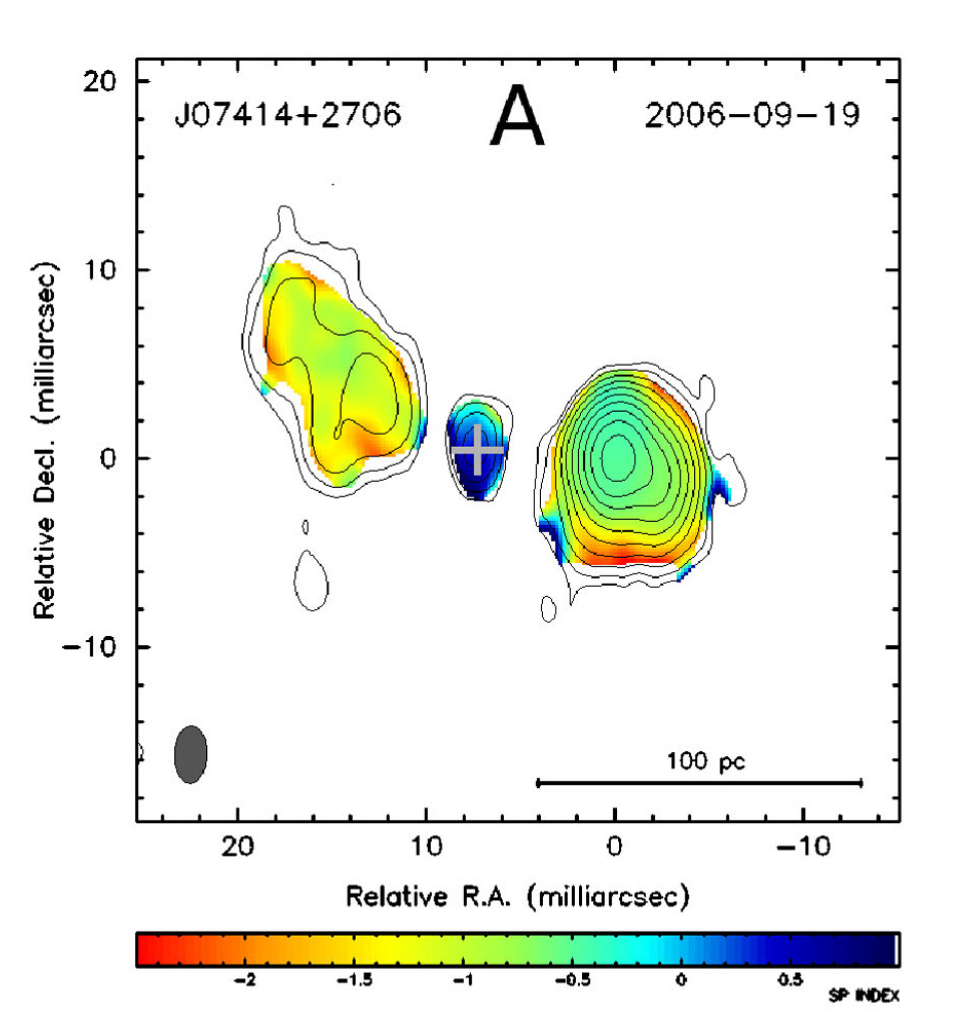
\includegraphics[width=.5\textwidth]{C:/Users/henri/OneDrive/Documents/NTNU/Semester 10/Masteroppgave/Plots/J0741+2706.png}
    \caption{The radio structure of CSO J0741+2706. The core is determined from the flat spectrum component and the symmetry of the radio lobes. Image taken from \cite{Tremblay_2016}}
    \label{fig:CSO_J0741}
\end{figure}

The last two criteria are the newest addition made by \cite{kiehlmann2023compact} and is the best way of separating CSOs from other jetted AGNs. The low variability and lack of relativisitic beaming has always been a key feature of CSOs, but since they were not included in the original classification there have been misidentification. An example quoted in \cite{kiehlmann2023compact} is the source PKS 1543+005 which shows strong variability and additionally the jet is projected on both sides of the core, giving the illusion of a compact double. With these new criteria one can be more certain that the sources in the catalogue are similar enough in nature to be able to make more general statements about them.





%\subsubsection*{Total energy density}
%The total energy density of the photon fields as a function of distance is then seen in figure \ref{fig:photon_fields}. Here one can see that the energy density of the photon fields is constant until the observer is outside the size of the respective regions. From the image it is clear that the biggest contributor to the total energy density becomes the IR torus, but all the regions contribute significantly to the total energy density.

%\subsubsection*{Spectral energy density}
%The spectral energy density of the different regions is of more interest since this is what will determine the effect of pion decay on protons accelerate in the jet or in the lobes. To create the 
%SED one has estimated the dynamical scale of our system and used the total photon densities to scale the SED accordingly. The resulting SED is seen in figure \ref{fig:SED_sep}. The SED are determined also on a number of 
%parameters, all which have taken from the literature. They are seen in table \ref{tab:SED_params}.

%The choice of variables comes from three sources. \cite{bronzini2024investigating} and \cite{kiehlmann2023compact} which both gives the disk luminosity of CSOs sources, and which we set to $10^{43} erg/s$. \cite{Ghisellini_2009} gives the rest of parameters that relate the different regions to the disk luminosity. The biggest caveat here is that these parameters are not specific to CSOs, but to Blazars in which they are based. For the purposes of this analysis one assumes that the parameters are the same for CSOs as for Blazars, and that one would not expect any significant difference. 

\begin{table}
    \centering
    \begin{tabular}{|c|c|}
        \hline
        Parameter & Value \\
        \hline
        $L_{d}$ & $10^{43}$ erg/s \\
        $GM$ & $G 10^{8} M_{\odot}$ \\
        $RS$ & $\frac{2GM}{c^2}$ \\
        $\eta$ & 0.1 \\
        $f_{X}$ & 0.3 \\
        $R_{X}$ & 30$ RS $\\
        $\beta$ & 0.4 $c$\\
        $f_{\text{BLR}}$ & 0.1 \\
        $R_{\text{BLR}}$ & $10^{17} \sqrt{L_{d}/10^{45}}$ cm \\
        $f_{\text{IR}}$ & 0.5 \\
        $R_{\text{IR}}$ & $2.5 10^{18}\sqrt{L_{d}/10^{45}}$ cm \\
        $\Gamma$ & 1.1 \\
        \hline
    \end{tabular}
    \caption{Parameters used to determine the SED of the different regions.}
    \label{tab:SED_params}
\end{table}
\begin{figure}
    \centering
    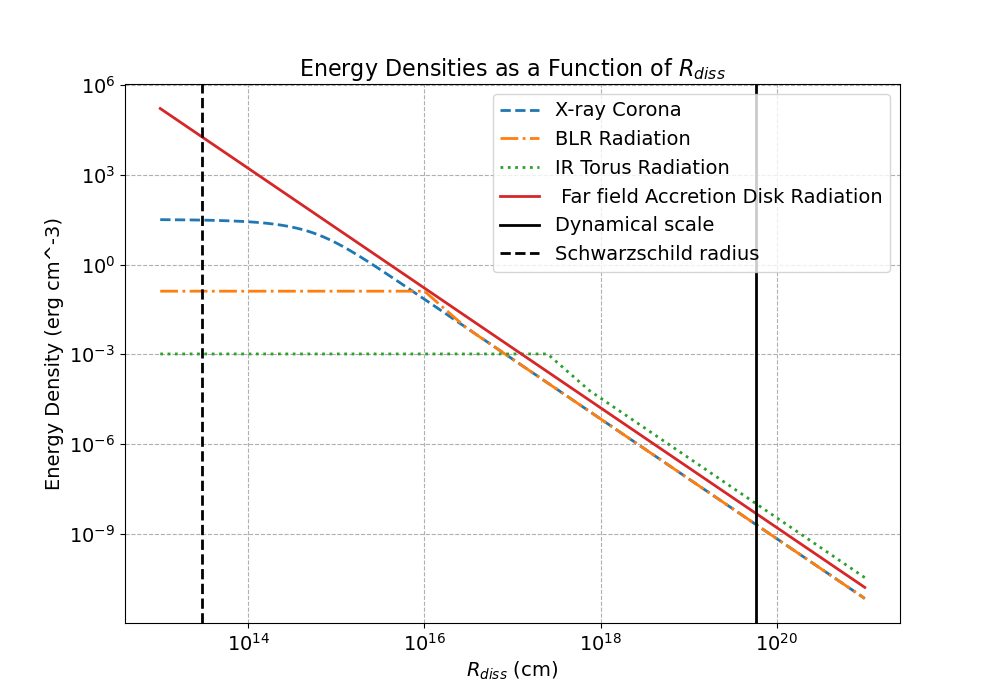
\includegraphics[width=.5\textwidth]{C:/Users/henri/OneDrive/Documents/NTNU/Semester 10/Masteroppgave/Plots/Energy_densities.png}
    \caption{The total energy density of the photon fields as a function radius from central engine.}
    \label{fig:photon_fields}
\end{figure}


\begin{figure}
    \centering
    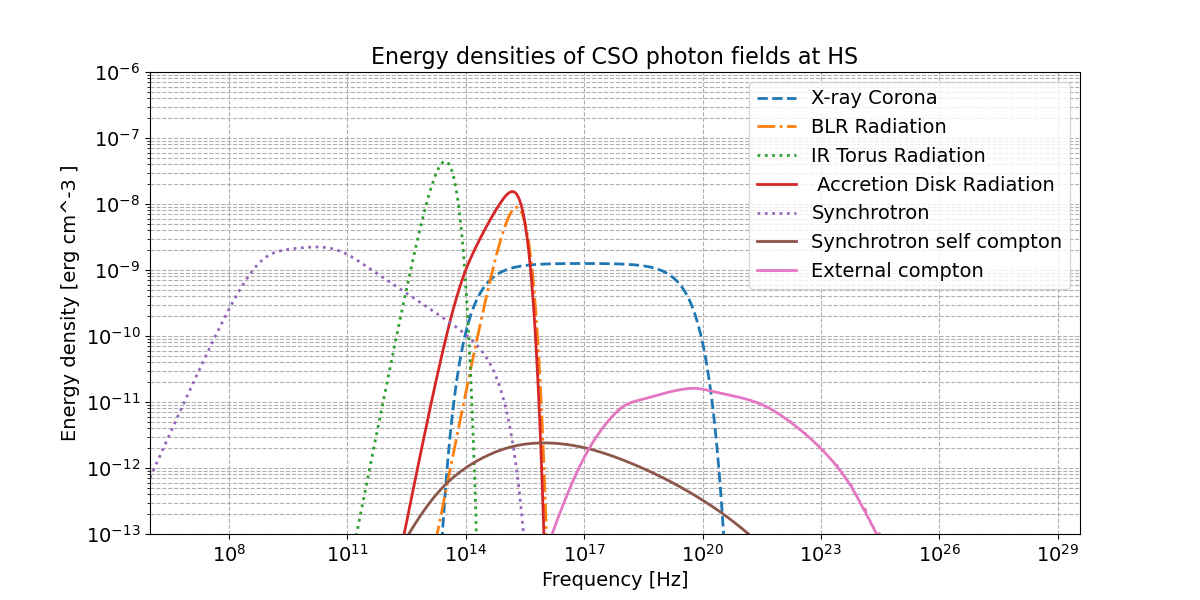
\includegraphics[width=.5\textwidth]{C:/Users/henri/OneDrive/Documents/NTNU/Semester 10/Masteroppgave/Plots/SEDs_sep.png}
    \caption{The spectral energy density at distance R}
    \label{fig:SED_sep}
\end{figure}

\begin{figure}
    \centering
    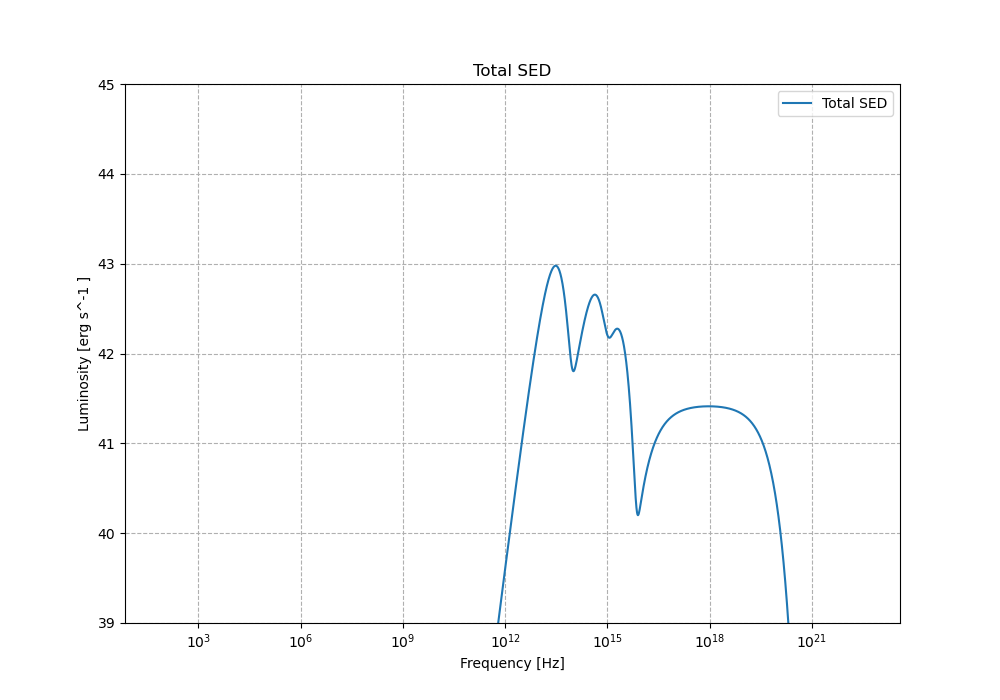
\includegraphics[width=.5\textwidth]{C:/Users/henri/OneDrive/Documents/NTNU/Semester 10/Masteroppgave/Plots/SED.png}
    \caption{Luminosity of the different components of the CSO that are close by the central engine. Missing synchrotron and IC part which is most prominent }
    \label{fig:Lum_SED}
\end{figure}

\subsection{Sub Classification of CSO}
Moving further along the classification of CSOs one now realises that there are two types of CSOs. CSO 2 and CSO 1. In CSO 2 sources one consider it edge brightened where there is significant luminosity in the radio lobes compared to the core. In CSO 1 sources one consider it edge dimmed where the luminosity of the radio lobes are significantly lower than that of the core. The origin of the two types of CSOs are thought to be the same, where CSO 1s represent failed CSO 2s. One will get back to the origin later in the report.

The fact of the matter is that also the CSO 2 class can further be subdivided. This extra subdivsion into CSO 2.0, 2.1, and 2.2 is on the basis of its morphology. In the number of Compact symmetric objects which succeed into becoming CSO 2s will go through different phases all with different characteristics. In figure \ref{fig:CSO_2_morphology} one can visualise the different phases of CSO 2 sources. The phases can analogously be compared to the different phases of shock evolution in supernovae.

\begin{figure}
    \centering
    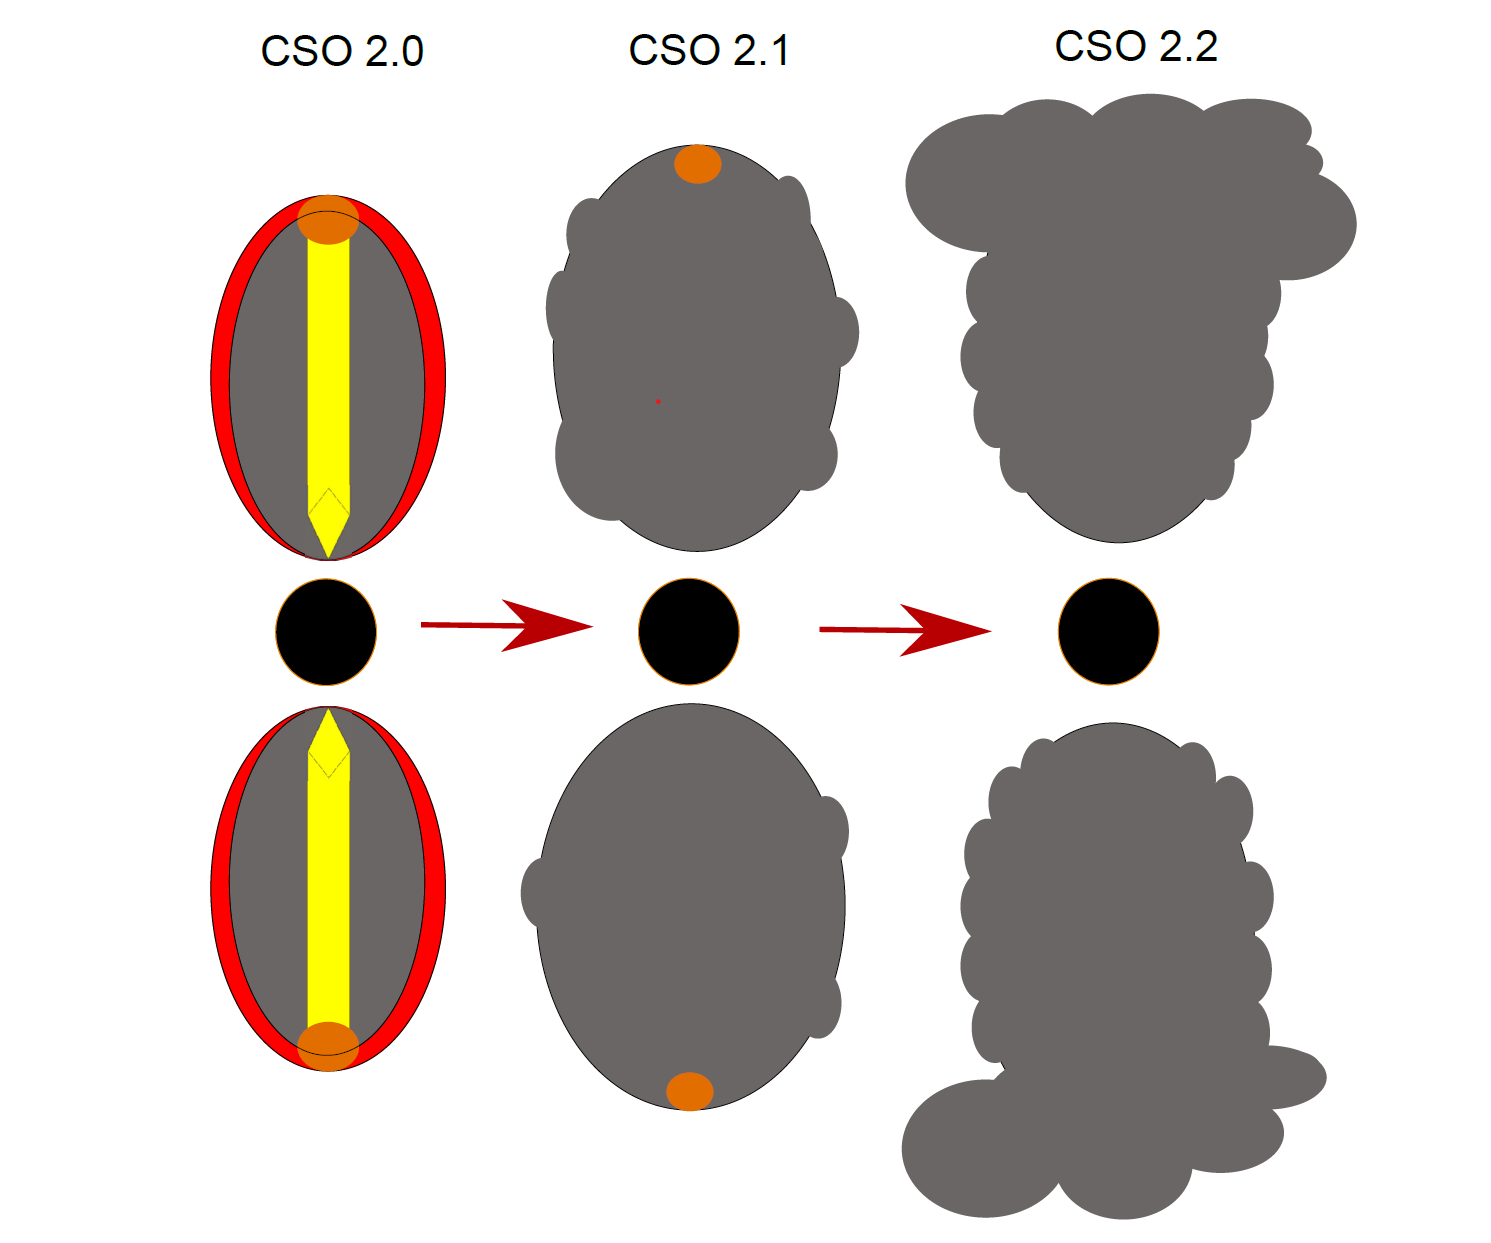
\includegraphics[width=.8\textwidth]{C:/Users/henri/OneDrive/Documents/NTNU/Semester 10/Masteroppgave/Plots/CSO_morphology.png}
    \caption{The different phases of CSO 2 sources. Image taken from \cite{sullivan2024smallscale}}
    \label{fig:CSO_2_morphology}
\end{figure}

\textbf{CSO 2.0}: According to \cite{sullivan2024smallscale} the CSO 2.0 phase evolves analogously to FRII radio galaxies. The edge-brightened lobes which contain prominent hot spots are similar to typical features of a relativitic jet pushing into the ambient medium. As \cite{sullivan2024smallscale} points out, classical jet models entail the jet collides with the ambient medium and forms two shock front, the forward shock and the reverse shock. From shock models the jet power $L_j$ is what determines the velocity of the forward shock, and in \cite{sullivan2024smallscale} the shock model used gives values similar to observation of CSO 2.0 lobe velocity($v_c = 0.2c$) and mach number of approximately $200$.

\textbf{CSO 2.1}: The mid life or CSO 2.1 is the transition of relativistic jet propagation into the sonic of subsonic regime. The category is often hard to define and is often contaminated by a  mix of CSO 2.0 and CSO 2.2. Nevertheless, it remains a separate category since there is still power in the hotspots and the lobes continue to expand but decelerate. 

\textbf{CSO 2.2}: The late life of CSOs or CSO 2.2 is the phase where the jet has decelerated to transonic speeds and the lobes are no longer expanding vertically as a result of jet pressure. The lobes are still expanding due to convectively rising turbulent plumes. When the plumes and the ambient densities are equal the lobes will stop expanding vertically and start expanding horizontally. \cite{sullivan2024smallscale} compares it to the characteristic mushroom cloud of volcanic which in this author's opinion paints a very nice image. 

This separation of CSOs will become important since certain enviroments are more favourable for the production of UHECRs and neutrinos. The most promising candidate are CSO 2.0 sources since they have the highest jet power and the highest velocity of the lobes. 

\subsection{Origin of CSOs/Fueling}
According to \cite{readhead2023compact} a possible method of fueling these objects is through tidal disruption events. Due to the short lifetime of these objects continued discrete fueling events become a good candidate for the ignition of the jets. Energetically one would assume that one needs a massive star to be able to fuel the CSO $2$ jets, but it is argued in \cite{sullivan2024smallscale} that this might not be the only solution. They argue that smaller mass stars which encounter the black hole could have sufficient magnetic flux to ignite the extraction of the black holes angular momentum. The method proposed in \cite{Blandford_1977} relate the extraction of black hole angular momentum  to the jet power via 

\begin{equation}
    L_j = \frac{1}{6\pi c} \Omega_{BH}^2 \Phi_{BH}^2
\end{equation}

After the TDE one expects the magnetic flux to disperse around the BH as $\Phi_{BH} \approx \Phi_{\star} \left(\frac{R_{H}}{R_{p}}\right)^2$ where $R_{H}$ is the black hole horizon and $R_{p}$ is the pericenter radius of the stellar encounter. In addition, the magnetic field could be amplified via strong dipolar dynamo action or magneto-rotational instability. The magnetic field could be strong enough to match the jet powers one observes in CSOs today even though the original stellar mass was low.The caveat here is that amplification of the magnetic field is required to reach sufficient levels.  


%It is argued in \cite{sullivan2024smallscale} that the introduction of external magnetic flux into an already existing seed field, created by possibly the accretion disk will lead to amplification of the magnetic field through extration of black hole angular momentum, \cite{Blandford_1977}. 

Along with the energetics one can put simple tests on this hypothosis by looking at the fallback time of debris onto a central black hole. This is also done in \cite{sullivan2024smallscale} which quote the fallback time as 

\begin{equation}
    t_f = 0.5 \text{yr}\left(\frac{M_{\rm BH}}{10^8 M_{\odot}}\right)^{1/2}\left(\frac{M_\star}{M_{\odot}}\right)^{-1}\left(\frac{R_\star}{R_{\odot}}\right)^{3/2}
\end{equation}

For the TDE hypothesis to be correct one would expect the fallback time to be of the order of the lifetime of the CSO 2.0, which is $t_f \approx 1000$ years. From the equation above red giants become a good candidate as they have a large radius and a low mass, and with a SMBH of $10^8 M_{\odot}$ the fallback time is of the order of $1000$ years.

Small sizes and finite lifetime are good indicators for transient events, and this is quoted in \cite{sullivan2024smallscale}


%From the papers of \cite{kiehlmann2023compact} to \cite{readhead2023compact}, and from \cite{sullivan2024smallscale} there is a clear quite new classification of CSOs. The classification is based on firstly CSOs being edge brightened or edge dimmed. Edge brightened sources which will onwards be refered as CSO 2s are bright in radio in their lobes, and CSO 1s or edge dimmed are thought to be CSOs that have stalled. 

%The big picture on CSOs is that they are a group of very short-lived sources that are ignited by transient events. Saying if the ignition of their jets are due to transient event such as tidal disruption event are covered in \cite{sullivan2024smallscale} and for the purposes of this study not necessary to discuss, but start a very interesting conversation. CSOs are then symmetric with the expansion of their jets into the interstellar medium visible from radio telescope. The symmetry of the jets is a key feature of CSOs and makes them unique in the sense of jetted-AGN since they have little to no features of relativistic beaming.   


\subsection{Catalouge of Bona fide CSO}
With the new criterias for CSOs \cite{kiehlmann2023compact} begun compiling a bone fide list of Compact symmetric objects. This new catalogue will serve as the testing grounds for their ability to produce UHECRs and neutrinos. The catalogue is a list of 79 sources which are somewhat split between the four different subclasses as seen in table \ref{tab:CSO_class} where only the CSO with a spectroscopic redshift have been given a class. The full source catalogue is listed in table \ref{tab:CSO_sources}.
%In order to study these sources there will always be a need for observational data. This fact combined with the fact that CSOs are a somewhat new class of AGN mean that there are no large catalogues of pure CSOs, and that many other catalogues misnomer sources as CSOs. This chapter will rely heavilly on \cite{kiehlmann2023compact} in which this is discussed and where they define a bona fide catalogue of 79 CSOs. The catalogue will allow us as it has in this paper to say more concrete information about the sources we are studying.
\begin{table}[H]
    \centering
    \caption{Catalouge of bona fide CSOs. Data taken from \cite{kiehlmann2023compact}}
    \label{tab:CSO_sources}
    \begin{tabular}{@{}ccccccccc@{}}
        \toprule
        ID & R.A. & Dec. & z & Ang\_size & Lin\_size & $\nu_t$ & $S_\nu$ & Class \\ \midrule
        J0000+4054 & 00:00:53.08 & +40:54:01.81 & nan & 124.0 & nan & 0.323 & 2.06 & nan \\
        J0003+4807 & 00:03:46.04 & +48:07:04.14 & nan & 16.2 & 0.139 & 2.123 & 0.348 & nan \\
        J0029+3456 & 00:29:14.24 & +34:56:32.25 & 0.517 & 29.1 & 0.180 & 0.8 & 2.0 & 2.1 \\
        J0111+3906 & 01:11:37.32 & +39:06:28.10 & 0.66847 & 8.0 & 0.056 & 4.0 & 1.33 & 2.0 \\
        J0119+3210 & 01:19:35.00 & +32:10:50.06 & 0.0602 & 100.0 & 0.115 & 0.4 & 4.0 & 2.2 \\
        J0131+5545 & 01:31:13.82 & +55:45:12.98 & 0.003649 & 23.0 & 0.016 & 0.657 & 0.31 & 2.2 \\
        J0132+5620 & 01:32:20.45 & +56:20:40.37 & nan & 12.2 & 0.104 & 3.42 & 0.6 & nan \\
        J0150+4017 & 01:50:19.61 & +40:17:30.02 & nan & 103.0 & 0.882 & 0.4 & 2.0 & nan \\
        J0204+0903 & 02:04:34.76 & +09:03:49.26 & nan & 33.0 & 0.282 & 1.3 & 2.0 & nan \\
        J0237+4342 & 02:37:01.21 & +43:42:04.18 & nan & 120.0 & nan & 0.3 & 0.868 & nan \\
        J0402+8241 & 04:02:12.68 & +82:41:35.13 & nan & 72.0 & 0.616 & 0.4 & 0.4 & nan \\
        J0405+3803 & 04:05:49.26 & +38:03:32.24 & 0.05505 & 42.0 & 0.044 & 0.07 & 5.5 & 2.0 \\
        J0425-1612 & 04:25:53.57 & -16:12:40.23 & nan & 99.8 & 0.854 & 0.363 & 1.449 & nan \\
        J0427+4133 & 04:27:46.05 & +41:33:01.10 & nan & 7.0 & 0.060 & 3.3 & 0.74 & nan \\
        J0440+6157 & 04:40:46.90 & +61:57:58.57 & nan & 30.0 & 0.257 & 1.7 & 0.24 & nan \\
        J0706+4647 & 07:06:48.07 & +46:47:56.45 & nan & 63.0 & 0.539 & 0.777 & 1.81 & nan \\
        J0713+4349 & 07:13:38.16 & +43:49:17.21 & 0.518 & 35.0 & 0.217 & 1.9 & 2.09 & 2.0 \\
        J0735-1735 & 07:35:45.81 & -17:35:48.50 & nan & 28.8 & 0.246 & 1.4 & 3.0 & nan \\
        J0741+2706 & 07:41:25.73 & +27:06:45.42 & 0.772139 & 26.0 & 0.193 & 1.0 & 1.05 & 2.0 \\
        J0754+5324 & 07:54:15.22 & +53:24:56.45 & nan & 26.0 & 0.223 & 1.24 & 0.634 & nan \\
        J0825+3919 & 08:25:23.68 & +39:19:45.76 & 1.21 & 70.7 & 0.591 & 0.517 & 1.77 & 2.1 \\
        J0832+1832 & 08:32:16.04 & +18:32:12.12 & 0.154 & 30.7 & 0.081 & 1.5 & 1.2 & 1 \\
        J0855+5751 & 08:55:21.36 & +57:51:44.09 & 0.025998 & 75.0 & 0.039 & 0.3 & 1.5 & 2.1 \\
        J0906+4124 & 09:06:52.80 & +41:24:30.00 & 0.0273577 & 11.1 & 0.006 & 1.5 & 0.06 & 1 \\
        J0909+1928 & 09:09:37.44 & +19:28:08.30 & 0.027843 & 14.7 & 0.008 & 6.0 & 0.12 & 1 \\
        J0943+1702 & 09:43:17.23 & +17:02:18.97 & 1.601115 & 20.4 & 0.175 & 4.0 & 0.4 & 2.0 \\
        J1011+4204 & 10:11:54.18 & +42:04:33.38 & nan & 115.0 & 0.984 & 0.424 & 1.16 & nan \\
        J1025+1022 & 10:25:44.20 & +10:22:30.00 & 0.045805 & 19.8 & 0.018 & 1.0 & 0.09 & 1 \\
        J1035+5628 & 10:35:07.04 & +56:28:46.79 & 0.46 & 38.0 & 0.221 & 1.3 & 1.87 & 2.0 \\
        J1042+2949 & 10:42:36.51 & +29:49:45.15 & nan & 45.0 & 0.385 & 0.7 & 1.0 & nan \\
        J1111+1955 & 11:11:20.07 & +19:55:36.01 & 0.299 & 15.5 & 0.068 & 1.305 & 1.1 & 2.0 \\
        J1120+1420 & 11:20:27.81 & +14:20:54.97 & 0.362 & 101.0 & 0.507 & 0.5 & 3.89 & 2.0 \\
        J1135+4258 & 11:35:55.99 & +42:58:44.65 & nan & 29.0 & 0.248 & 1.0 & 1.45 & nan \\
        J1148+5924 & 11:48:50.36 & +59:24:56.36 & 0.01075 & 54.8 & 0.012 & 6.149 & 0.573 & 1 \\
        J1158+2450 & 11:58:25.79 & +24:50:18.00 & 0.203 & 46.0 & 0.152 & 2.0 & 1.25 & 2.2 \\
        J1159+5820 & 11:59:48.77 & +58:20:20.31 & 1.27997 & 70.2 & 0.591 & 0.6 & 1.9 & 2.0 \\
        J1204+5202 & 12:04:18.61 & +52:02:17.62 & nan & 54.0 & 0.462 & 0.7 & 1.4 & nan \\

        \bottomrule
    \end{tabular}
\end{table}

\begin{table}
    \centering
    \begin{tabular}{@{}ccccccccc@{}}
        \toprule
        ID & R.A. & Dec. & z & Ang\_size & Lin\_size & $\nu_t$ & $S_\nu$ & Class \\ \midrule
        J1205+2031 & 12:05:51.50 & +20:31:19.00 & 0.02378857 & 22.0 & 0.010 & 1 & 0.14 & 2.1 \\
        J1220+2916 & 12:20:06.82 & +29:16:50.72 & 0.002 & 46.8 & 0.002 & 0.074 & 0.65 & 1 \\
        J1227+3635 & 12:27:58.72 & +36:35:11.82 & 1.975 & 58.8 & 0.499 & 1.2 & 2.14 & 2.0 \\
        J1234+4753 & 12:34:13.33 & +47:53:51.24 & 0.373082 & 27.4 & 0.140 & 1.4 & 0.36 & 2.1 \\
        J1244+4048 & 12:44:49.19 & +40:48:06.15 & 0.813586 & 70.0 & 0.529 & 0.405 & 2.03 & 2.2 \\
        J1247+6723 & 12:47:33.33 & +67:23:16.45 & 0.107219 & 5.0 & 0.010 & 1.16 & 0.36 & 2.0 \\
        J1254+1856 & 12:54:33.27 & +18:56:01.93 & 0.1145 & 4.14 & 0.008 & 6.0 & 0.13 & 1 \\
        J1311+1658 & 13:11:23.82 & +16:58:44.22 & 0.081408 & 27.0 & 0.041 & 0.447 & 0.824 & 1 \\
        J1313+5458 & 13:13:37.85 & +54:58:23.91 & 0.613 & 57.0 & 0.384 & 0.555 & 1.65 & 2.2 \\
        J1326+3154 & 13:26:16.51 & +31:54:09.52 & 0.36801 & 68.0 & 0.345 & 0.5 & 7.03 & 2.2 \\
        J1335+5844 & 13:35:25.93 & +58:44:00.29 & nan & 12.9 & 0.110 & 4.9 & 0.9 & nan \\
        J1347+1217 & 13:47:33.36 & +12:17:24.24 & 0.121 & 100.0 & 0.215 & 0.4 & 8.86 & 2.2 \\
        J1400+6210 & 14:00:28.65 & +62:10:38.59 & 0.431 & 67.6 & 0.378 & 0.5 & 6.56 & 2.2 \\
        J1407+2827 & 14:07:00.40 & +28:27:14.69 & 0.077 & 11.0 & 0.016 & 4.9 & 3.0 & 2.1 \\
        J1413+1509 & 14:13:41.66 & +15:09:39.51 & nan & 15.0 & 0.128 & 2.5 & 0.47 & nan \\
        J1414+4554 & 14:14:14.85 & +45:54:48.73 & 0.186 & 30.5 & 0.094 & 0.693 & 0.396 & 2.1 \\
        J1416+3444 & 14:16:04.18 & +34:44:24 & nan & 81.0 & 0.693 & 0.7 & 2.1 & nan \\
        J1434+4236 & 14:34:27.86 & +42:36:20.06 & 0.452 & 68.3 & 0.393 & 0.074 & 1.67 & 2.2 \\
        J1440+6108 & 14:40:17.87 & +61:08:42.88 & 0.445365 & 30.0 & 0.171 & 0.4 & 0.48 & 2.1 \\
        J1443+4044 & 14:42:59.32 & +40:44:28.94 & nan & 123.4 & nan & 0.292 & 1.55 & nan \\
        J1508+3423 & 15:08:05.70 & +34:23:23.00 & 0.045565 & 280.0 & 0.247 & 0.23 & 0.25 & 2.1 \\
        J1511+0518 & 15:11:41.27 & +05:18:09.26 & 0.084 & 10.6 & 0.017 & 0.4 & 0.48 & 2.0 \\
        J1559+5924 & 15:59:01.70 & +59:24:21.84 & 0.0602 & 11.0 & 0.013 & 0.15 & 0.23 & 1 \\
        J1602+5243 & 16:02:46.38 & +52:43:58.40 & 0.105689 & 250.0 & 0.478 & 0.15 & 1.48 & 1 \\
        J1609+2641 & 16:09:13.32 & +26:41:29.04 & 0.473 & 61.3 & 0.362 & 1.1 & 5.44 & 2.1 \\
        J1645+2536 & 16:44:59.07 & +25:36:30.64 & 0.588 & 39.0 & 0.258 & 1.0 & 1.1 & 2.1 \\
        J1723-6500 & 17:23:41.03 & -65:00:36.61 & 0.01443 & 7.0 & 0.002 & 2.7 & 4.48 & 2.1 \\
        J1734+0926 & 17:34:58.38 & +09:26:58.26 & 0.735 & 12.8 & 0.093 & 2.3 & 1.22 & 2.0 \\
        J1735+5049 & 17:35:49.01 & +50:49:11.57 & 0.835 & 8.0 & 0.061 & 6.4 & 0.972 & 2.0 \\
        J1816+3457 & 18:16:23.90 & +34:57:45.75 & 0.245 & 45.5 & 0.174 & 0.44 & 0.983 & 2.1 \\
        J1826+1831 & 18:26:17.71 & +18:31:52.89 & nan & 74.0 & 0.633 & 0.308 & 1.08 & nan \\
        J1826+2708 & 18:26:32.11 & +27:08:07.95 & nan & 41.0 & 0.351 & 1.0 & 0.34 & nan \\
        J1915+6548 & 19:15:23.82 & +65:48:46.39 & 0.486 & 36.0 & 0.216 & 0.5 & 0.83 & 2.1 \\
        J1928+6815 & 19:28:20.55 & +68:14:59.27 & nan & 128.1 & nan & 0.074 & 1.04 & nan \\
        J1939-6342 & 19:39:25.02 & -63:42:45.62 & 0.183 & 42.6 & 0.130 & 1.4 & 15.0 & 2.0 \\
        J1944+5448 & 19:44:31.51 & +54:48:07.06 & 0.263 & 48.8 & 0.196 & 0.778 & 1.77 & 2.0 \\
        J1945+7055 & 19:45:53.52 & +70:55:48.73 & 0.101 & 40.6 & 0.075 & 1.8 & 0.929 & 2.2 \\
        J2022+6136 & 20:22:06.68 & +61:36:58.80 & 0.2266 & 29.0 & 0.104 & 4.086 & 2.64 & 2.1 \\
        J2203+1007 & 22:03:30.95 & +10:07:42.59 & 1.005 & 11.0 & 0.089 & 4.427 & 0.306 & 2.0 \\
        J2327+0846 & 23:27:56.70 & +08:46:44.30 & 0.02892 & 1300.0 & 0.744 & 0.09 & 1.0 & 1 \\
        J2347-1856 & 23:47:08.63 & -18:56:18.86 & nan & 33.4 & 0.186 & 1.8 & 0.66 & nan \\
        J2355+4950 & 23:55:09.46 & +49:50:08.34 & 0.23831 & 90 & 0.337 & 0.7 & 2.93 & 2.2 \\
        \bottomrule

     
    \end{tabular}
\end{table}


\begin{table}
    \caption{Classification of CSOs in the catalogue.}
    \label{tab:CSO_class}
    \centering
    \begin{tabular}{@{}ccc@{}}
        \toprule
        Class & Number of sources & Percentage of total  \\ \midrule
        CSO 1 & 11 & 20.4  \\
        CSO 2.0 & 17 & 31.5  \\
        CSO 2.1 & 15 & 27.8  \\
        CSO 2.2 & 11 & 20.4  \\
        \bottomrule
    \end{tabular}
\end{table}
\newpage

\subsection{Characteristic of CSOs vs linear size}
Radio luminosity is a key feature of CSOs, is a good indicator of magnetic field strength, and allows us 
to probe the radio lobes of CSOs. In figure \ref{fig:Luminosity_size} one can see the radio luminosity at peak frequency of CSOs as a function of linear size. 

\begin{figure}
    \centering
    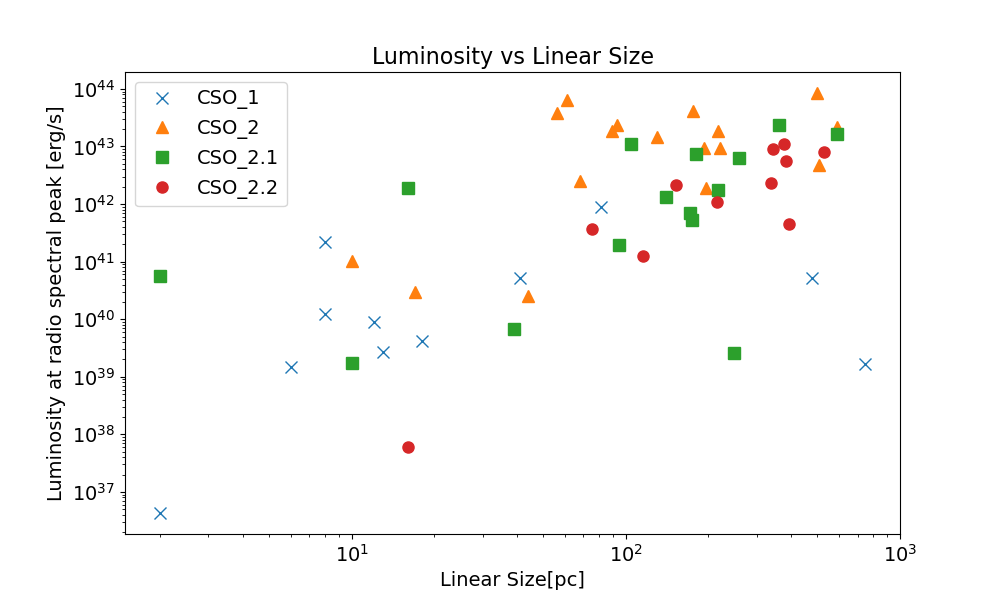
\includegraphics[width=.8\textwidth]{C:/Users/henri/OneDrive/Documents/NTNU/Semester 10/Masteroppgave/Plots/Lin_size_vs_Luminosity.png}
    \caption{The radio luminosity at peak frequency of CSOs as a function of linear size.}
    \label{fig:Luminosity_size}
\end{figure}

The figure shows a distinction between CSO $2.0$ and the other classes where CSO $2.0$ have a higher luminosity at peak frequency compared to the other classes of similar sizes. In addition one sees a trend of higher luminosity at the peak frequency for larger sources. This is expected since the amount of energy deposited into the lobes will 
 affect the size of the lobes.

One can also investigate the relation between redshift and luminosity at peak frequency as seen in figure \ref{fig:Luminosity_redshift}. Here one sees a trend of higher luminosity at peak frequency for higher redshifts, indicating a possible obersvation bias for longer distances.



\begin{figure}
    \centering
    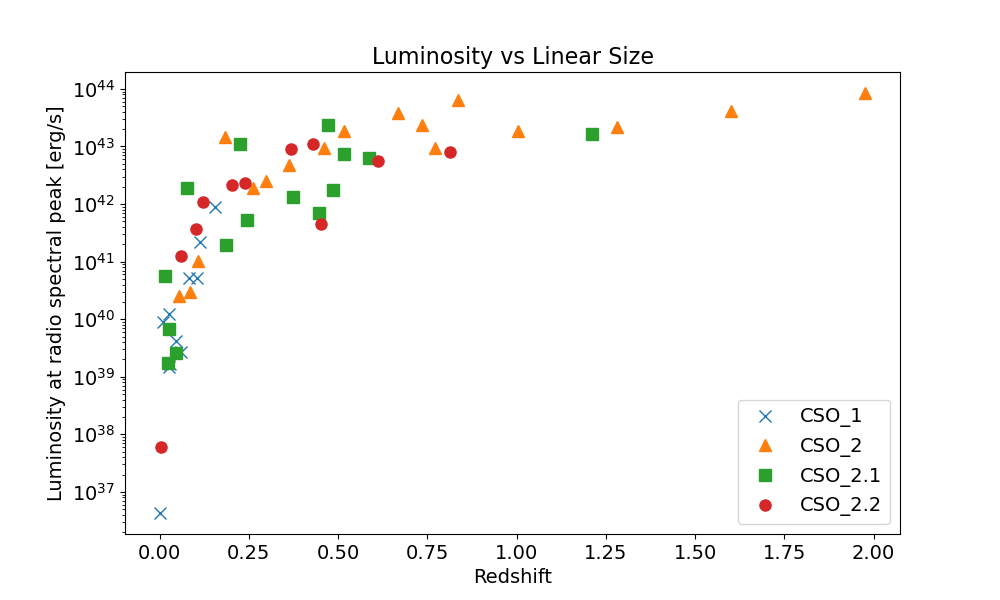
\includegraphics[width=.8\textwidth]{C:/Users/henri/OneDrive/Documents/NTNU/Semester 10/Masteroppgave/Plots/z_vs_Luminosity.png}
    \caption{The radio luminosity at peak frequency of CSOs as a function of redshift.}
    \label{fig:Luminosity_redshift}
\end{figure}
\subsection{Prevalence of CSOs}







%\subsection{Stability in jet expansion and lobes.} The most promesing feature of CSOs which we will see as a key feature in the section on time-scales is the stability of the lobes in radio emission, the stability of the jet expansion and the stability of most wavelengths in emissions. In \cite{bronzini2024investigating} they report no significant variablilty of one CSO source in gamma rays, variability of the order of years in x-ray, with the broadband SED showing variability on the timescales of years. This is a clear distincsion from other jetted AGN which are known to be highly variable. Having stable systems allows for more efficient acceleration of ions, and significantly increases the possibility of producing UHECRs. 
\newpage
\printbibliography
\end{document}
